\chapter{Deterministic RL-MPC}
\label{chapter:deterministic_RL_MPC}
This chapter aims to construct the RL-MPC framework and examines various implementations to determine their effectiveness. The resulting controllers are evaluated by comparing them with the MPC and RL controllers developed in previous sections. The implementations serve as a means to understand the construction of the final RL-MPC algorithm, as each subsequent implementation builds on the previous one. In addition, this chapter will analyse the nominal case in which the parameters of the model and environment are known.


\section{Implementation} \label{section:rlmpc implementation}
Although there are numerous implementations of RL-MPC, limited research focuses on maximising economic benefit specifically for continuous state and action spaces while training RL separately from MPC. As stated in \citet{ellisTutorialReviewEconomic2014} and \citet{amritEconomicOptimizationUsing2011}, an EMPC without a terminal constraint and terminal cost function does not provide performance and stability guarantees. Specifically, \citet{ellisTutorialReviewEconomic2014} states that a terminal point constraint is required to ensure closed-loop performance, while \citet{amritEconomicOptimizationUsing2011} extends this concept by proving that applying a terminal region constraint with an appropriate terminal cost function is required to guarantee closed-loop performance.\citet{amritEconomicOptimizationUsing2011} further claims that the terminal cost function with a terminal region constraint is superior to the terminal point constraint because it increases the size of the feasible set of initial conditions and may possibly improve the closed-loop performance. However, finding such suitable terminal constraints and cost functions proves to be very difficult. The objective of this thesis is to ascertain whether the RL agent is capable of providing this. \\
Furthermore, when considering the RL perspective in these implementations, it is important to note that the learned value function is merely an approximation. Consequently, when this value function is used in MPC, it is effectively unrolled, and value iterations are executed. This process can result in an improved policy compared to the original policy that generated the value function.

The integration of RL into MPC will increasingly involve more complex implementations to analyse the impact at each stage. Firstly, initial guesses provided from the actor will be examined. Subsequently, the RL agent will establish a terminal point constraint. Following this, the RL agent will define and determine a terminal region constraint. The various value functions trained by the nominal agent (\autoref{tab:various-vf}) will then be used as the terminal cost function, with and without the terminal region constraint. Lastly, a parallel problem will be presented to explore a slightly alternative application of the value function. The integration of the value function into the MPC’s optimal control is facilitated by L4Casadi \cite{salzmannLearningCasADiDatadriven2023,salzmannRealtimeNeuralMPCDeep2023}.

\subsection{RL-MPC problem formulations}

\paragraph{RL-MPC 1}
Implementation of RL-MPC 1 is identical to \autoref{eq:mpc_ocp} but includes initial guesses provided by RL. However, instead of using the previous solution to the state and input trajectories as initial guesses, the RL agent provides these initial guesses. Two sets of initial guesses will be tested and compared with one another. The solution to the OCP in \autoref{eq:mpc_ocp} at time $k$ can be denoted as:

\begin{equation}\label{eq:sol-mpc-ocp}
	\begin{aligned}
		&\mathbf{x}_{k|k} = [x_{k|k},x_{k_+ 1|k},x_{k + 2|k}, ...,x_{k + N_p|k}]^T \\ 
		&\mathbf{u}_{k|k} = [u_{k|k},u_{k + 1|k}, ...,u_{k + N_p-1|k}]^T \\
	\end{aligned}
\end{equation}

The two sets of initial guesses at the $k$ step is denoted as:

\begin{equation}\label{eq:initial-guess-1}
	\begin{aligned}
		&\tilde{\mathbf{x}}_{k|k} = [\tilde{x}_{k|k},\tilde{x}_{k+1|k},...,\tilde{x}_{k + N_p|k}]^T \\ 
		&\tilde{\mathbf{u}}_{k|k} = [\tilde{u}_{k|k},\tilde{u}_{k + 1|k},...,\tilde{u}_{k + N_p - 1|k}]^T\\ 
	\end{aligned}
\end{equation}

\begin{equation}\label{eq:initial-guess-2}
	\begin{aligned}
		&\hat{\mathbf{x}}_{k|k} = [\hat{x}_{k|k},\hat{x}_{k+1|k},...,\hat{x}_{k + N_p|k}]^T \\ 
		&\hat{\mathbf{u}}_{k|k} = [\hat{u}_{k|k},\hat{u}_{k + 1|k},...,\hat{u}_{k + N_p - 1|k}]^T\\ 
	\end{aligned}
\end{equation}

such that

 \begin{equation}\label{eq:horizon_extension}
 	\begin{aligned}
 		&\tilde{\mathbf{x}}_{k|k} = [\mathbf{x}_{k|k-1},f(x_{k-1 + N_p|k-1}, \pi(x_{k-1 + N_p|k-1}), d_{k+Np|k},p)]^T\\ 
 		&\tilde{\mathbf{u}}_{k|k} = [\mathbf{u}_{k|k-1},\pi(x_{k-1 + N_p|k-1})]^T\\
 	\end{aligned}
 \end{equation}

\begin{equation}\label{eq:actor_roll_out}
	\begin{aligned}
		&\hat{\mathbf{x}}_{k|k} = [x_{k|k},f(x_{k|k},\pi(x_{k|k}),d_{k|k},p),..., f(x_{k+N_p-1|k}, \pi(x_{k + N_p-1|k}), d_{k_1 + Np-1|k},p)]^T \\ 
		&\hat{\mathbf{u}}_{k|k} = [\pi(x_{k|k},\pi(x_{k+1|k}),...,\pi(x_{k+Np-1|k})]^T \\ 
	\end{aligned}
	\end{equation}

\autoref{eq:horizon_extension} takes the previous time steps solution, shifts it in time and uses the policy $\pi(\cdot)$, as provided by the actor, to calculate the optimal action and resulting state to take at the last time step. This method can be interpreted as extending the horizon. So, for every time step, the initial guesses of the sequence of actions and states are extended by one time step from the previous solution. \autoref{eq:actor_roll_out} unrolls the RL policy $\pi(\cdot)$ from the current state until the end of the prediction horizon. Consequently, the solutions obtained from the previous time, $\mathbf{x}_{k|k}$ and $\mathbf{u}_{k|k}$, step are disregarded, thus generating a new sequence without relying on the previous time step’s solutions. It must be noted that, for the first time step, $k=0$, initial guesses given by \autoref{eq:initial-guess-2} are used for both cases, therefore $\tilde{x}_{k|k} \leftarrow \hat{x}_{k|k}$ and $\tilde{u}_{k|k} \leftarrow \hat{u}_{k|k}$.

Based on prior analyses, generating these initial guesses is extremely fast. Furthermore, since it comes from a policy comparable to the MPC’s, these initial guesses can be used for more than just initial guesses, but also to generate terminal constraints. The subsequent implementations explore the significance of these initial guesses, particularly the initial guesses mentioned in \autoref{eq:initial-guess-1}.

\paragraph{RL-MPC 2}
RL-MPC 2 incorporates a terminal point constraint in addition to the initial guesses. \citet{risbeckEconomicModelPredictive2020}, \citet{amritEconomicOptimizationUsing2011}, proves that an appropriate terminal constraint can result in superior performance. It is shown that, through this terminal constraint, for a time-varying system, performance can be guaranteed to be as least as good as a reference trajectory, $(\mathbf{x}_r, \mathbf{u}_r)$, that serves as a basis for a meaningful economic performance for the system. The terminal constraint should be imposed to keep the system close to this reference trajectory. Since the RL policy can be used as the reference policy, it can be guaranteed that the resulting policy will be at least as good as the RL policy. The asymptotic average performance of the EMPC can be guaranteed to be no worse than the performance of a reference trajectory under the following assumptions from \citet{amritEconomicOptimizationUsing2011,risbeckEconomicModelPredictive2020}:

\hspace{1cm} \textbf{Assumption 1} (Properties of constraint sets) The set $\mathbb{Z}$ is compact, where $\mathbb{Z} \subseteq \mathbb{X} \times \mathbb{U}$

\hspace{1cm} \textbf{Assumption 2}  (Continuity of cost and system) The functions $l(\cdot), f(\cdot)$ are continuous on $\mathbb{Z}$. The terminal cost function $V_f(\cdot)$ is continuous on $\mathbb{X}_f$ 

\hspace{1cm} \textbf{Assumption 3}  The reference trajectory $(\mathbf{x}_r, \mathbf{u}_r)$ satisfies $f(x_r(k),u_r(k),d(k),p)=x_r(k+1)$

\hspace{1cm} \textbf{Assumption 4} (Stability assumption) There exist a compact terminal region $\mathbb{X}_f \subseteq \mathbb{X}$, containing the point $x_r$ in its interior, and control law $\kappa_f : \mathbb{X}_f \rightarrow \mathbb{U}$, such that the following holds 
\begin{equation}\label{eq:assumption_3}
	V_f(f(x,\kappa_f(x))) \leq V_f(x) - l(x,\kappa_f(x)) + l(x_r(t),u_r(t)) \quad \forall x \in \mathbb{X}_f
\end{equation}

Assumptions 1, 2, and 3 hold since all states and inputs are bounded and the stage cost, as defined in \autoref{eq:mpc_stage_cost}, is continuous. For this implementation,$V_f(\cdot) \equiv 0$ since no terminal cost function is used. Assumption 3 holds if $x,\kappa_f(x)$ is constrained to $x_r,u_r$. Therefore, if the terminal state was constrained to the last initial guess of \autoref{eq:initial-guess-1}, it would constrain it to the RL’s reference policy. Therefore, the terminal constraint would be imposed on the last state of the solution such that:

\begin{equation}\label{eq:terminal-constraint-ocp}
\begin{aligned}
	&x_{k+Np|k} = \tilde{x}_{k+Np|k}\\ 
	&u_{k+Np-1|k} = \tilde{u}_{k+Np-1|k}\\
\end{aligned}
\end{equation}

Nevertheless, this implementation is also evaluated for initial guesses provided by \autoref{eq:initial-guess-2}. However, it is important to note that, because the reference trajectory depends on the current state it therefore changes at each time step. No meaningful comparison can be made to this changing reference trajectory. So, while it will perform at least as well as this changing reference trajectory, the performance on this changing trajectory is unknown.

\paragraph{RL-MPC 3}
RL-MPC 3 builds upon RL-MPC 2, in that instead of providing a terminal point constraint, a terminal region constraint as provided by the \autoref{eq:initial-guess-1} and \autoref{eq:initial-guess-2} is used. The terminal region is defined as:

\begin{equation}\label{eq:terminal-region}
	\begin{aligned}
		& (1-\epsilon)\tilde{x}_{k+Np|k} \leq x_{k+Np|k} \leq (1+\epsilon)\tilde{x}_{k+Np|k}\\
		&(1-\epsilon)\tilde{u}_{k+Np-1|k} \leq u_{k+Np-1|k} \leq (1+\epsilon) \tilde{u}_{k+Np-1|k}\\
	\end{aligned}
\end{equation}

where $\epsilon$ is expressed as a percentage, allowing the terminal state to fall within a predefined range around the terminal guess. \cite{amritEconomicOptimizationUsing2011} suggests that this has the same performance guarantees as RL-MPC 2 under the same assumptions. However introducing a terminal region for the terminal state makes it difficult to meet assumption 4 from \autoref{eq:assumption_3}. However, \cite{amritEconomicOptimizationUsing2011} suggest that providing a terminal region may be more beneficial than a terminal constraint since more freedom is given to the EMPC. Finally, a terminal constraint and initial guesses will also be provided by \autoref{eq:initial-guess-2} to investigate performance. However, since unrolling from the current state does not result in following a fixed trajectory, no meaningful performance comparisons can be made to the RL agent (i.e. the reference trajectory).

\paragraph{RL-MPC 4}
RL-MPC 4 only includes the value function learned in \autoref{section:trained-vf} and initial guesses given in \autoref{eq:initial-guess-1}. This implementation examines the effect of the value function on the performance of the resulting controller. The value function can be incorporated into \autoref{eq:mpc_ocp} by defining a cost function:

\begin{equation}\label{eq:cost-function}
		\min_{u(k),x(k)}  \sum_{k = k_0}^{k_0 + N_p - 1}{l(u(k), y(k))} - V_{\phi_i}(s'(k_0 + N_p))
\end{equation}

where $V_{\phi_i}$ represents the learned value function and $s'(k_0+N_p)$ is the normalisation of $s(k_0+N_p)$, as per \autoref{eq:state-normalization}. For $V_{\phi_1}$,$V_{\phi_2}$ and $V_{\phi_3}$, $s(\cdot)$ is the observation returned by the agent ( \autoref{eq:obs-tuple-1}), while $s(\cdot)$ when using $V_{\phi_4}$ is $(y_{k_0+N_p},k_0+N_p)$ as discussed in \autoref{section:trained-vf}. This implementation aims to evaluate the impact of different neural network architectures, including: a deep neural network ($V_{\phi_1}$), a smaller deep neural network ($V_{\phi_2}$), a shallow neural network ($V_{\phi_3}$), and a reduced-order deep neural network trained to learn the value function using only two system states ($V_{\phi_4}$). According to approximate dynamic programming as stated in \cite{bertsekasLessonsAlphaZeroOptimal}, this policy could be better than the policy that generated the value function. However, the performance is heavily dependent on the quality of the value function. If the approximate value function is inaccurate and the errors are significant and systematic, then unrolling this value function could lead to a worse policy. This can be considered a naive implementation of RL-MPC. It can be conceptually viewed as either unrolling the value function and subsequently performing a minimisation or providing the MPC knowledge of the future, essentially extending its prediction horizon. Note that the value function is maximised by minimising the negative of the value function, since it represents total return and not cost.

\paragraph{RL-MPC 5}
The implementation of RL-MPC 5 essentially combines RL-MPC 3 and RL-MPC 4. \citet{amritEconomicOptimizationUsing2011} states that finding an appropriate terminal cost function and corresponding terminal region proves non-trivial  to satisfy assumption 3. This implementation is also claimed to be superior to the terminal point constraint of implementation RL-MPC 2 \cite{amritEconomicOptimizationUsing2011}. Furthermore, RL-MPC 5 provides additional knowledge of the future rewards to be expected compared to RL-MPC 3; therefore, an increase in performance over RL-MPC 3 can be expected. Therefore, the resulting RL-MPC OCP is defined as:

\begin{subequations} \label{eq:rl-mpc-ocp}
	\begin{align}
		\min_{u(k),x(k)} & \sum_{k = k_0}^{k_0 + N_p-1} {l(u(k), y(k))} - V_{\phi_4}(s'(k_0+N_p)) \\
		\text{s.t.} \quad & x(k+1) = f(x(k), u(k), d(k), p),  \label{eq:rl-mpc-dynamics-constraint} \\
		& y(k) = g(x(k+1), p), \label{eq:rl-mpc-output-constraint} \\
		& -\delta u \leq u(k) - u(k-1) \leq \delta u, \label{eq:rl-mpc-delta-u} \\
		& u_{\min} \leq u(k) \leq u_{\max}, \label{eq:rl-mpc-u-limits}\\
		& x(k_0) = x_{k_0}. \label{eq:rl-pmc-initial} \\
 		&\tilde{\mathbf{x}}_{k|k} = [\mathbf{x}_{k|k-1},f(x_{k-1 + N_p|k-1}, \pi(x_{k-1 + N_p|k-1}), d_{k+Np|k},p)]^T\\ 
		&\tilde{\mathbf{u}}_{k|k} = [\mathbf{u}_{k|k-1},\pi(x_{k-1 + N_p|k-1})]^T\\
		& (1-\delta_T)\tilde{x}_{k+Np|k} \leq x_{k+Np|k} \leq (1+\delta_T)\tilde{x}_{k+Np|k}\\
		&(1-\delta_T)\tilde{u}_{k+Np-1|k} \leq u_{k+Np-1|k} \leq (1+\delta_T) \tilde{u}_{k+Np-1|k}\\
	\end{align}
\end{subequations}

This implementation was investigated to determine whether RL might provide an adequate terminal region and cost function to improve the MPC's performance and produce a high-performing EMPC. 


\paragraph{RL-MPC 6}
Implementation 6 is an alternative method of incorporating the value function. This implementation involves solving implementation 3; however, with \autoref{eq:initial-guess-1} ($\tilde{\mathbf{x}}_{k|k},\tilde{\mathbf{u}}_{k|k}$) and \autoref{eq:initial-guess-2} ($\hat{\mathbf{x}}_{k|k},\hat{\mathbf{u}}_{k|k}$) separately. Once solved, the terminal state of the two solution trajectories are compared by evaluating them with the value function. The solution trajectory with the terminal state that yields the highest value (given from the value function) is selected as the final solution, and the first control input of this solution is taken. It essentially selects the best policy. Although only two policies are compared, this method may warrant further research whereby multiple policies generate their own respective initial guesses and terminal region constraints and compared. The policies generated could originate from multiple RL agents, each providing their initial estimations and with corresponding terminal constraints. Although each problem could be solved in parallel to speed up computational speed, it was implemented sequentially in this thesis.



\subsection{Initial RL and MPC performance}
A review of the RL, $\pi(\cdot)$, and MPC,$\kappa(\cdot)$, policies are evaluated for the nominal conditions.


\begin{figure}[H]
	\centering
	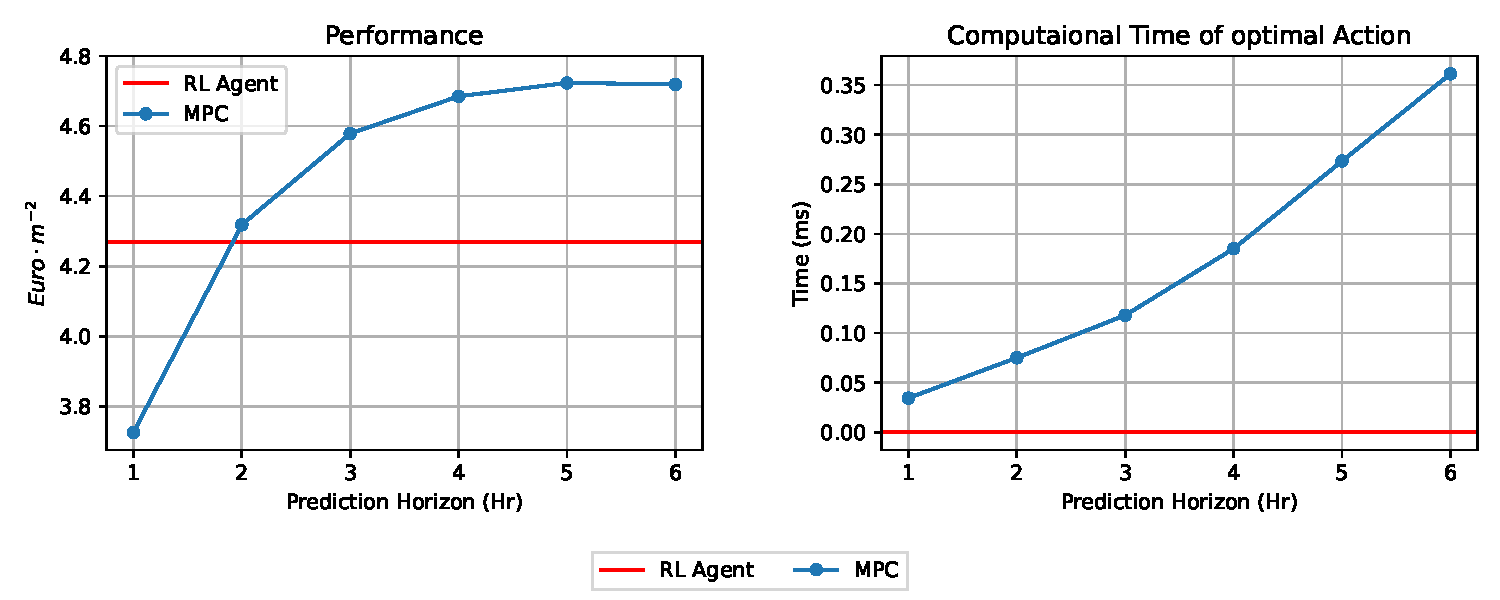
\includegraphics[width=\textwidth]{figures/mpc_vs_rl_nominal.pdf}
	\caption{MPC vs RL in nominal conditions}
	\label{fig:rl-vs-mpc-nominal}
\end{figure}


\autoref{fig:rl-vs-mpc-nominal} demonstrates the performance of the MPC and RL agent in the nominal setting. It was previously thought that MPC would be myopic in this economic optimisation setting, however it achieves relatively high performance and outperforms RL. While the RL agent's performance is inferior to MPC for all prediction horizons (except 1 hour), it should not be assumed that this is the best RL policy available.  RL can potentially generate an improved policy by conducting a more thorough hyper-parameter tuning. Additionally, with a discount factor ($\gamma = 0.95$) set at such a high value, RL should be capable of considering a longer time horizon beyond 6 hours. A more extensive hyper-parameter tuning may have to be done to achieve a policy that outperforms MPC. However, the RL agent is competitive and, as seen in \autoref{fig:rl-vs-mpc-nominal}, can compute actions significantly faster. It is evident that the RL agent can be used to generate a reference trajectory for RL-MPC with minimal increase in computational time. The performance of the resulting RL-MPC and its potential superiority will be analysed in the following sections and compared to the baseline performances, as depicted in \autoref{fig:rl-vs-mpc-nominal}. 

The RL-MPC was initially developed to aid MPC in its short sightedness by providing it information about the system past its prediction horizon. However MPC's performance can already be considered satisfactory. The deterministic RL-MPC framework was developed to determine whether information from RL can still help the MPC, specifically at shorter prediction horizons, in making better decisions. Therefore shorter prediction horizons may be used while keeping computational costs low and performance high. Once this has been determined, the RL-MPC framework will be tested in a stochastic environment to determine whether knowledge of the uncertainty present can be transferred to the RL-MPC from RL.

\section{Results - RL-MPC 1}
This implementation consists of passing in 2 sets of initial guesses for the MPC, namely \autoref{eq:initial-guess-1} ($\tilde{\mathbf{x}}_{k|k},\tilde{\mathbf{u}}_{k|k}$) and \autoref{eq:initial-guess-2} ($\hat{\mathbf{x}}_{k|k},\hat{\mathbf{u}}_{k|k}$).
\begin{figure}[H]
	\centering
	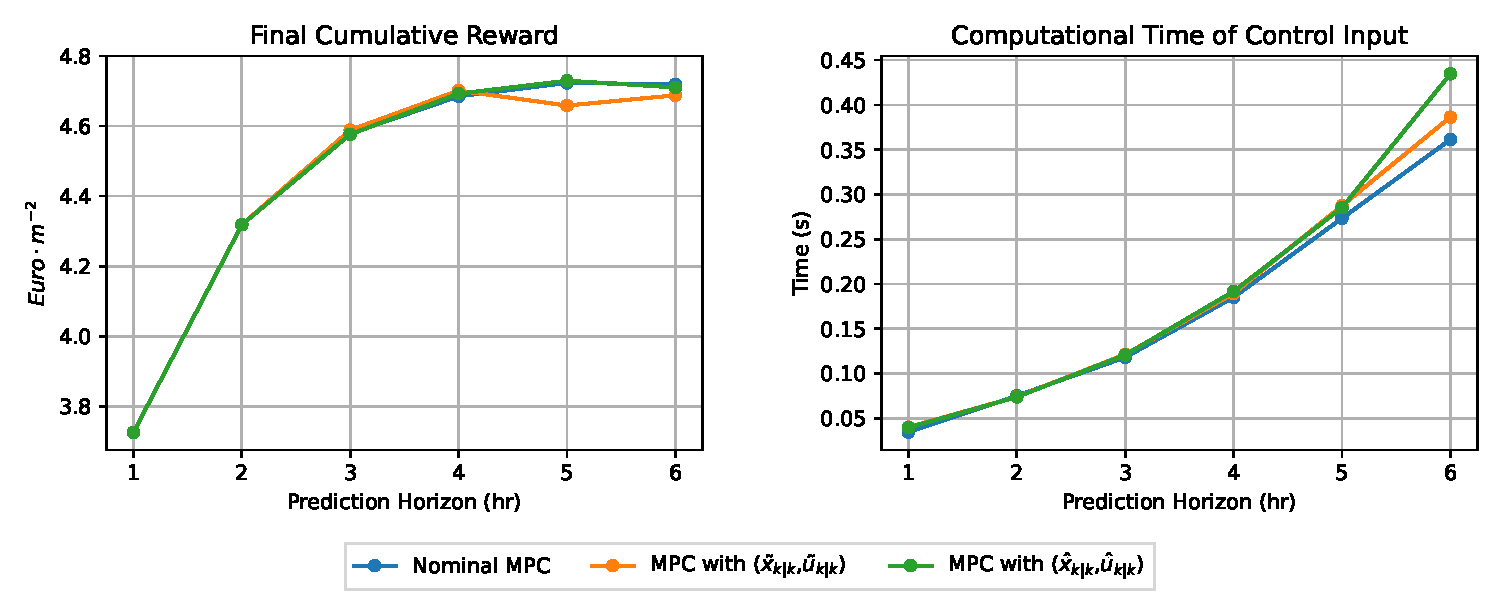
\includegraphics[width=\textwidth]{figures/rl_mpc_impl_1.pdf}
	\caption{MPC vs MPC with initial guesses}
	\label{fig:rlmpc-impl1}
\end{figure}

\autoref{fig:rlmpc-impl1} presents the results of passing in  these two sets of initial guesses. Using \autoref{eq:initial-guess-2} seems to have very little impact on the final cumulative reward; however, it increases the computational time of the control input at a 6 hour prediction horizon. This could be because the initial guesses are derived from a worse performing policy than MPC itself. Moreover, using \autoref{eq:initial-guess-1} also has minimal impact on the final cumulative reward. However, performance degrades significantly for a prediction horizon of 5 and 6 hours compared to the nominal MPC. Additionally, computational time also increases. A reason for the sub-optimal performance may be due to using the initial guesses of the Lagrangian multipliers found from the previous solution. The actor's initial guesses may differ significantly from the previous solution, rendering the Lagrangian multipliers' guesses nonsensical. While the actor may offer initial guesses, they are insufficient for improving or assisting the MPC, and simply using the previous solution as an initial guess may be more beneficial. However, the importance of having good initial guesses becomes more significant as the prediction horizon is extended and the problem complexity increases. Therefore, if a superior policy to the nominal MPC were to provide initial guesses instead of an inferior policy, it could result in a more favourable outcome.

\section{Results - RL-MPC 2}

\begin{figure}[H]
	\centering
	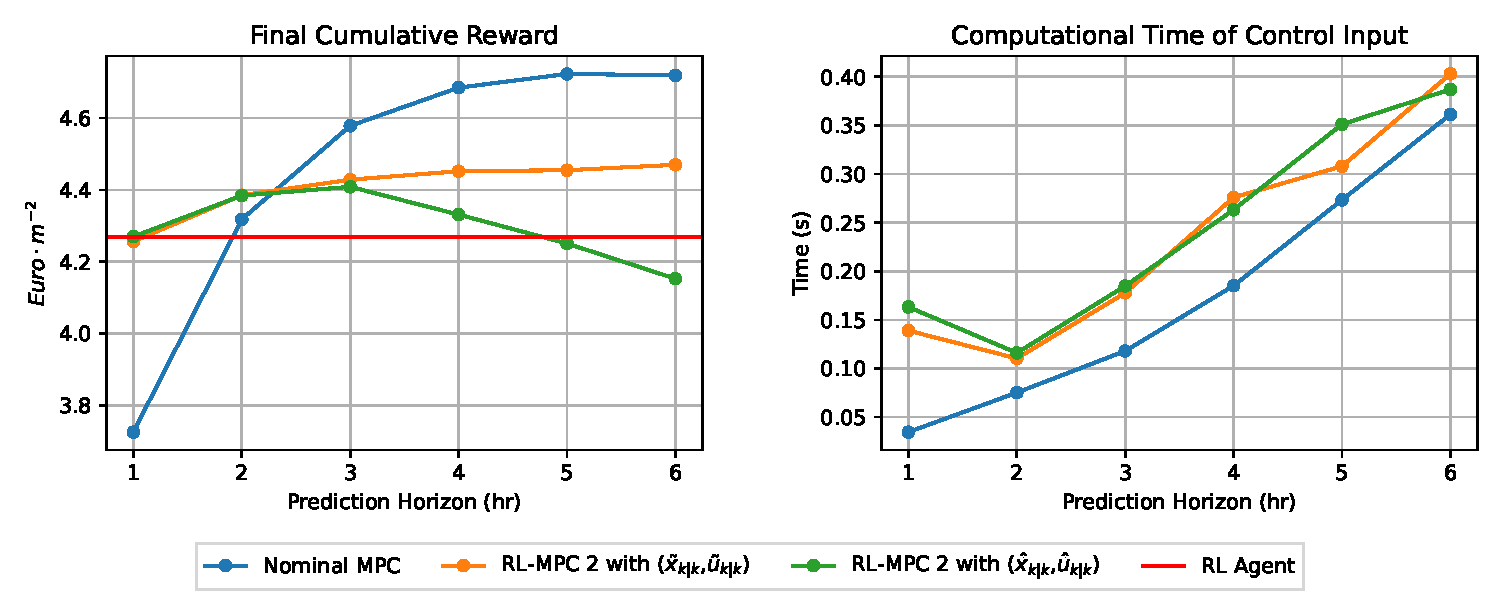
\includegraphics[width=\textwidth]{figures/rl_mpc_impl_2.pdf}
	\caption{MPC with terminal constraints from agent}
	\label{fig:rlmpc-impl2}
\end{figure}

The approach described in implementation RL-MPC 2 was used to guarantee that the RL-MPC policy achieves a performance level equal to or better than the RL policy. The performance of the resulting policies is illustrated in \autoref{fig:rlmpc-impl2}. It is evident that, for a terminal point constraint and initial guesses as given by \autoref{eq:initial-guess-1}, the resulting policy is at least as good as the RL's, even at lower prediction horizons where RL performs better than MPC. Nevertheless, the RL-MPC policy exhibits notably inferior performance to the MPC policy when the prediction horizon exceeds 3 hours. Beyond the 3-hour mark, the MPC policy consistently outperforms the RL and RL-MPC policies.  While implementing RL-MPC may enhance the RL policy, it does not guarantee that the resulting policy will surpass the policy generated purely by MPC. If the RL policy is more competitive and surpasses the performance of the MPC, then implementing this RL-MPC implementation would be advantageous, as is the case for a prediction horizon of 1 and 2 hours. This marks a very important design choice. One can choose to either impose a terminal point constraint to guarantee a certain level of performance or instead opt to extend the prediction horizon of the MPC until satisfactory performance is acquired. However, as mentioned, extending the horizon for the MPC controller does not guarantee better performance under economic optimisation. Therefore, a safer choice may be to implement the terminal point constraint provided by the RL agent.
\\
The lack of performance guarantees for the terminal point constraint and initial guesses, as indicated by equation \autoref{eq:initial-guess-2}, is evident in the decrease in performance, which becomes worse than RL when longer prediction horizons are considered.\\
The computational time for the control input significantly increases. The terminal constraint may be excessively limiting the MPC due to the presence of a sub-optimal terminal constraint, particularly when dealing with longer prediction horizons.

\section{Results - RL-MPC 3}
This implementation aims to move away from the terminal constraint and allow the MPC more freedom by providing it with a terminal region constraint as outlined in \autoref{eq:terminal-region}, with a chosen $\epsilon = 5\%$, allowing for a $10\%$ deviation in the terminal state around the terminal guess. As claimed in \cite{amritEconomicOptimizationUsing2011}, this could prove to be more beneficial than the terminal point constraint, provided that an appropriate cost function is supplied. For this implementation, the cost function supplied is effectively $V_f(\cdot) \equiv 0$. 


\begin{figure}[H]
	\centering
	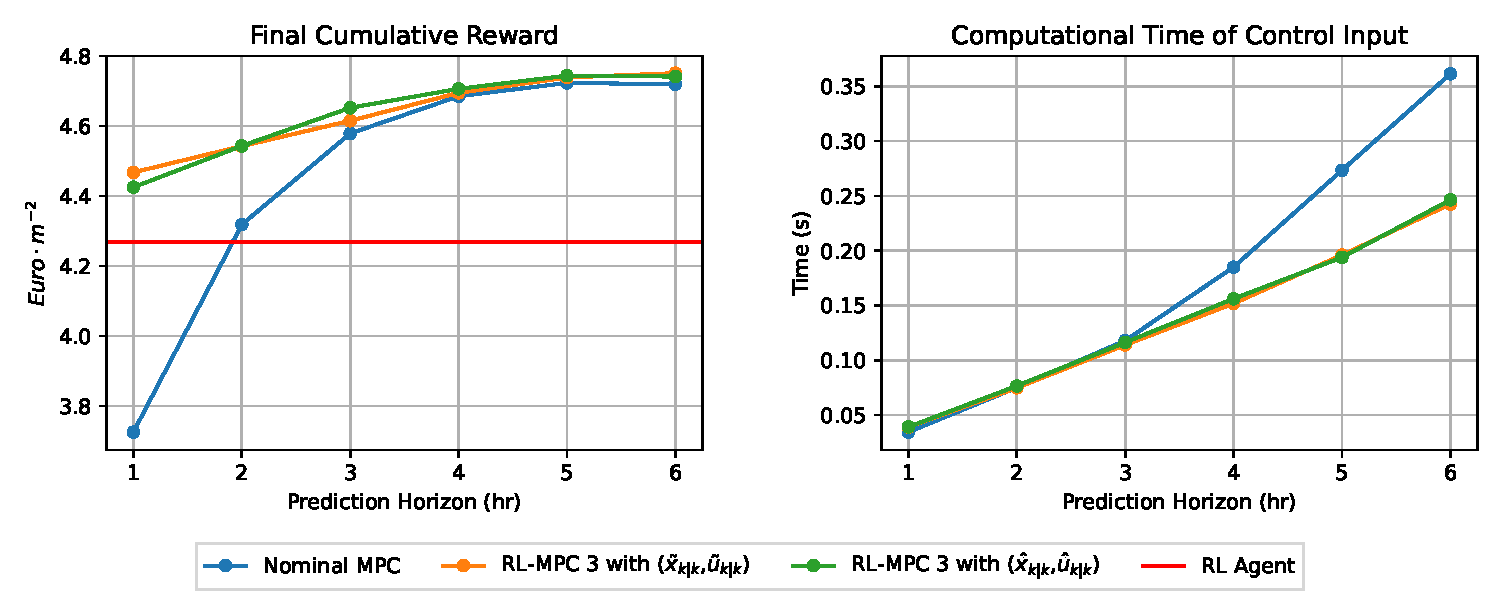
\includegraphics[width=\textwidth]{figures/rl_mpc_impl_3.pdf}
	\caption{MPC with terminal region}
	\label{fig:rlmpc-impl3}
\end{figure}

The results from the implementation are depicted in \autoref{fig:rlmpc-impl3}. Shortening the prediction horizons results in a substantial increase in the overall cumulative reward compared to the standalone MPC and RL policies. Furthermore, the RL-MPC obtains a marginally superior final cumulative reward compared to the MPC even at longer prediction horizons with both terminal regions generated from each set of initial guesses. Lastly, it appears that this performance is increasing monotonically with an increase in prediction horizon. This could indicate that an appropriate terminal region has been found to  guarantee performance and stability. However, longer prediction horizons would be required to provide conclusive evidence.\\

Additionally, this terminal region also allowed for a lower computation time of the control inputs, with a noticeably faster compute time at longer prediction horizons. This is likely because the terminal region is less limiting than the terminal constraint while also guiding the MPC, resulting in reduced computational times. It was noted that fewer instabilities in the solver were encountered at higher prediction horizons when using the terminal region constraint, which could be the reason for such a noticeable speedup. However, \autoref{fig:rlmpc-impl3} also indicates that the terminal region can be created using either a fixed reference trajectory ($(\tilde{\mathbf{x}}_{k|k}, \tilde{\mathbf{u}}_{k|k})$) or a changing one $(\hat{\mathbf{x}}_{k|k}, \hat{\mathbf{u}}_{k|k})$ to observe improvements in performance. 

It is noted that the resulting performance (increase in total cumulative reward and decrease in computational time) of the RL-MPC policy outperforms both standalone policies, even when the terminal region and initial guesses are supplied by a policy that performs substantially worse than the MPC controller. This underscores the necessity of giving certain future-oriented information to the EMPC to attain optimal economic advantage and performance. 

\section{Results - RL-MPC 4}
This implementation investigates the effect of supplying the MPC with a cost function, specifically an approximate value function represented by a neural network, $V_{\phi}$. Each value function, as listed in \autoref{tab:various-vf}, is tested as a terminal cost function for the MPC.


\begin{figure}[H]
	\centering
	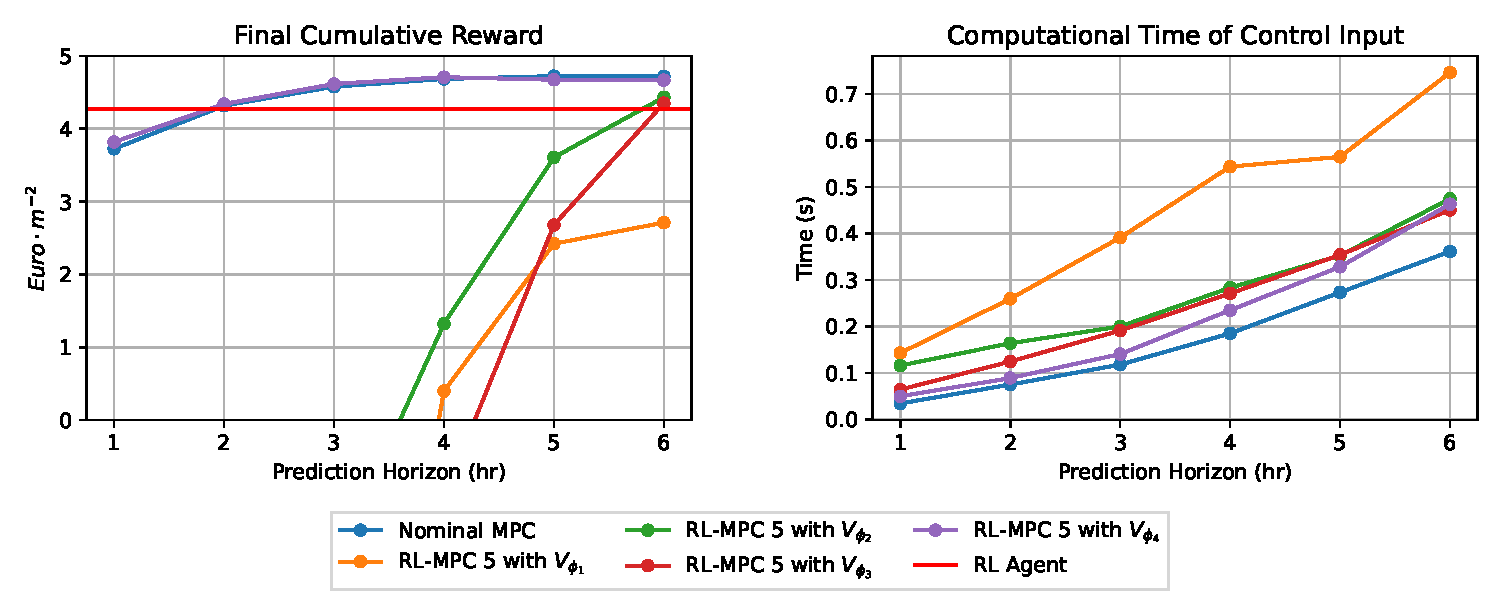
\includegraphics[width=\textwidth]{figures/rl_mpc_impl_4.pdf}
	\caption{MPC with terminal cost function that optimises over all terminal states}
	\label{fig:rlmpc-impl4-all-states}
\end{figure}

\autoref{fig:rlmpc-impl4-all-states} is a naive implementation of merging RL and MPC. As can be seen, the outcomes are unsatisfactory regarding the overall cumulative reward and the computational time required for generating control inputs. Caution must be exercised when employing a neural network in an optimiser, as they are an extremely non-linear. As illustrated in \autoref{fig:rlmpc-impl4-all-states}, the performance deteriorates further as the neural network becomes more complex. The neural networks exhibit highly non-convex behaviour that may cause the MPC optimiser to become easily trapped in local optima. The only value function that seems not to destabilize the optimiser is ${V}_{\phi_4}$ which is also the only value function that exhibits a smooth behaviour, see \cref{rem:vf-smoothness}. The MPC's optimisation task is solely focused on maximising the drymass in this particular value function, with time being a constant parameter. However, the MPC must optimise across all possible model states and inputs for the other value functions. \\
It is natural to observe an increase in computational time in \autoref{fig:rlmpc-impl4-all-states}. Once again, the highly non-convex nature of the behaviour can disrupt the MPC optimiser and lead to unpredictable computational times. However, the simpler the neural network's architecture, the more reduced the computational time. It is expected that even for a high quality value function such as $V_{\phi_4}$, adding a neural network to the optimisation problem will increase the computational burden due to the added complexity. Ultimately the results in \autoref{fig:rlmpc-impl4-all-states} highlight the significance of obtaining a high-quality value function.

\begin{figure}[H]
	\centering
	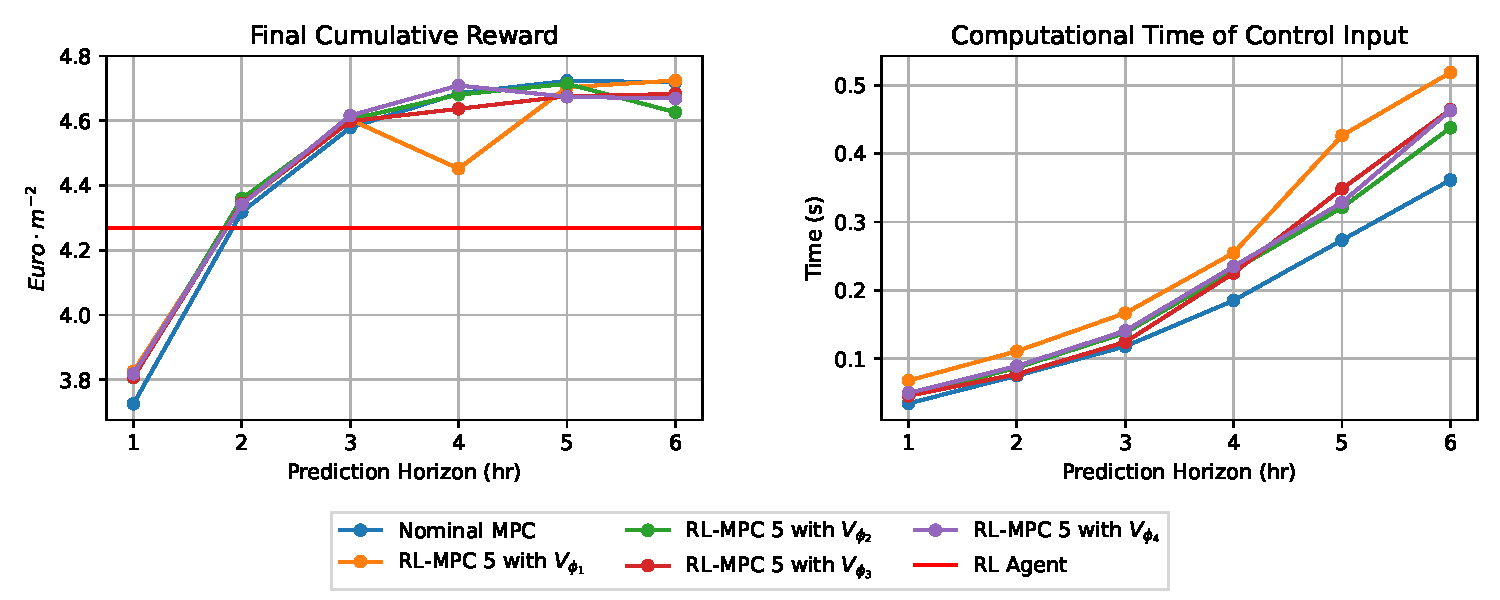
\includegraphics[width=\textwidth]{figures/rl_mpc_impl_4_1.pdf}
	\caption{MPC with terminal cost function that optimises over time and terminal dry mass}
	\label{fig:rlmpc-impl4-only-drymass}
\end{figure}

With the exception of the dry mass, all decision variables were constrained at their initial guesses to reduce the non-linearity of the value functions. This action was taken due to the clear indication that the value of a state can be reasonably approximated by considering the time and the state of the drymass, as explained in \autoref{section:trained-vf}. Therefore, the optimisation process for ${V}_{\phi_1}$, ${V}_{\phi_2}$, and ${V}_{\phi_3}$, which use a complete state observation (\autoref{eq:obs-tuple-1}) as inputs, was solely focused on optimising the dry mass input while keeping the other inputs fixed, similar to ${V}_{\phi_4}$.

The performance of the resulting RL-MPC policy is demonstrated in \autoref{fig:rlmpc-impl4-only-drymass}. Adding the value functions improves the final cumulative reward over MPC at shorter prediction horizons but degrades performance for longer prediction horizons (5 and 6 hours). Although the value functions have been simplified, increasing the prediction horizon still allows the MPC's optimisation to get trapped in local optima; this could be the reason for the observed performance degradation in \autoref{fig:rlmpc-impl4-only-drymass}. It is noted that the value functions contain information that the MPC can leverage, albeit resulting in only a slight performance increase when it does not destabilise the optimiser. Moreover, simplifying of the value function also resulted in more predictable times, with very little increase compared to the nominal MPC.\\

The performance of ${V}_{\phi_4}$ is superior to the others (at prediction horizons 1-4 hours) because it was trained exclusively on the drymass state and time, enabling it to make more accurate predictions of the value of a specific state using only these two inputs; therefore ${V}_{\phi_4}$ is used in the final implementation. These results suggest that a value function can increase performance over nominal MPC but not necessarily over the RL policy from which it was derived from. In addition, for the value function to be effective, it should have as few local optima as possible (i.e., it should have as low a degree of non-linearity as possible) while maintaining accuracy. Furthermore, it should be smooth and capable of generalising effectively across the state space to ensure reliable performance. Lastly, it is important to balance the performance gains with the increased computational time. Shown in \autoref{tab:rl-mpc-v4}, the increase in computational time far outweighs the marginal performance increase for shorter prediction horizons. However, combining it with a terminal region constraint may reduce computational times.

\begin{table}[H]
	\centering
	\begin{tabular}{|c|cccccc|}
		\hline
		&1hr&2hr&3hr&4hr&5hr&6hr\\
		\hline
		Final Cumulative Reward Increase(\%) &2.484 &0.525&0.814&0.512&-1.041& -1.069\\
		\hline
		Computational Time Increase     (\%) &50.888 &40.358&30.859&29.062&14.243& 23.013\\
		\hline
	\end{tabular}
	\caption{RL-MPC $\tilde{V}_4$ performance comparison compared to MPC}
	\label{tab:rl-mpc-v4}
\end{table}

\section{Results - RL-MPC 5 and 6}

Implementation of RL-MPC 5 aims to incorporate both a terminal region constraint and a terminal cost function. ${V}_{\phi_4}$ is used as a cost function with a terminal region generated by $(\tilde{\mathbf{x}}_{k|k},\tilde{\mathbf{u}}_{k|k})$ initial guesses as in \autoref{eq:initial-guess-1}, with an $\epsilon =5\%$. Implementation RL-MPC 6 solves two problems, each with its initial guesses ($(\tilde{\mathbf{x}}_{k|k},\tilde{\mathbf{u}}_{k|k})$ and $(\hat{\mathbf{x}}_{k|k},\hat{\mathbf{u}}_{k|k})$) that are used to construct each of the problem's terminal regions. After solving the two problems, the better policy is determined by evaluating the terminal state in each solution using the value function, ${V}_{\phi_4}$.

\begin{figure}[H]
	\centering
	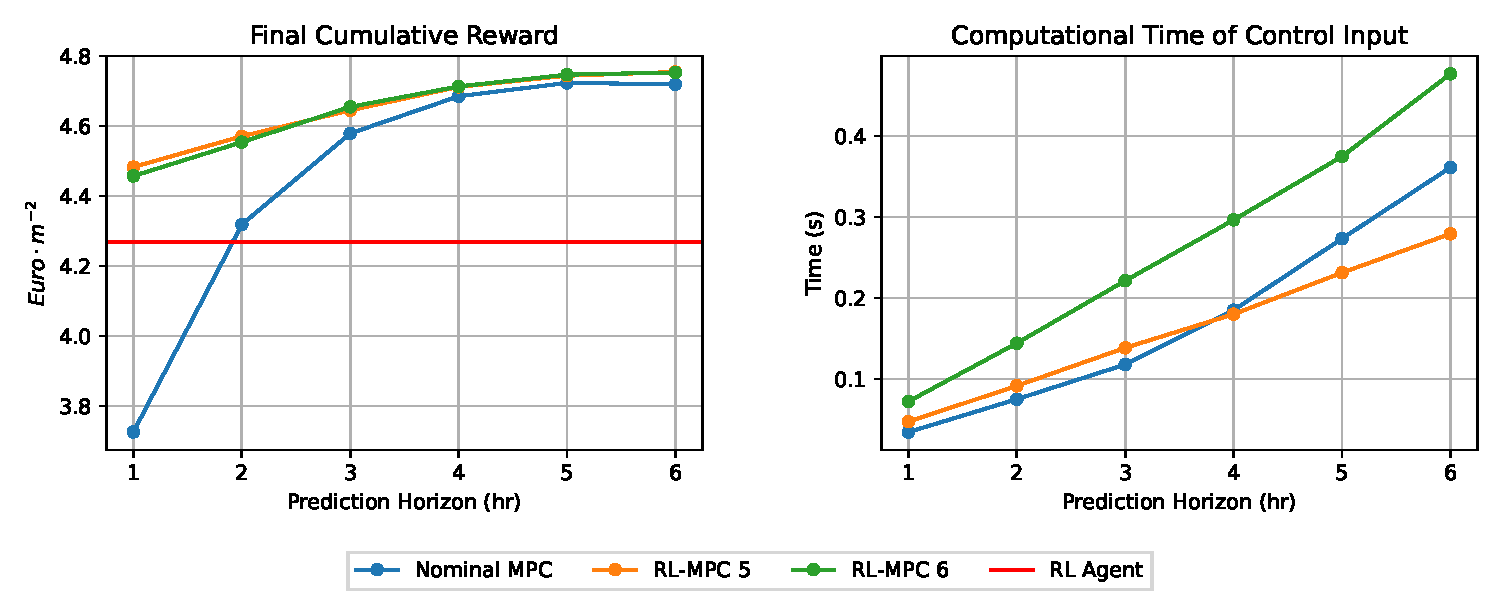
\includegraphics[width=\textwidth]{figures/rl_mpc_impl_5_6.pdf}
	\caption{MPC vs RL-MPC with terminal region and cost function vs RL-MPC solving two separate problems and evaluating best policy with value function}
	\label{fig:rlmpc-impl5-6}
\end{figure}

As demonstrated in \autoref{fig:rlmpc-impl5-6}, both implementations outperform the standalone MPC and RL policies across all MPC prediction horizons. The computational time of implementation RL-MPC 6 is notably higher because it solves two optimisation problems instead of just one. However, it is possible to solve the two problems in parallel, effectively reducing the computational time by half. Although the performance gains are substantial as compared to the standalone MPC, it is noted that the majority of this performance increase may be due to the terminal region constraint. Furthermore, despite including a neural network in the optimisation problem (RL-MPC 5), the computational time is reduced to a similar level as the standalone MPC when a terminal region constraint is present. Whether or not a cost function is necessary when a terminal region constraint has already improved performance so much is investigated in \autoref{section:final-rl-mpc-nominal}.

\section{Final Result and Conclusion} \label{section:final-rl-mpc-nominal}
The three best implementations are compared, namely RL-MPC 3 (with $\tilde{x}_{k|k}$,$\tilde{u}_{k|k}$), RL-MPC 5 and 6.
\begin{figure}[H]
	\centering
	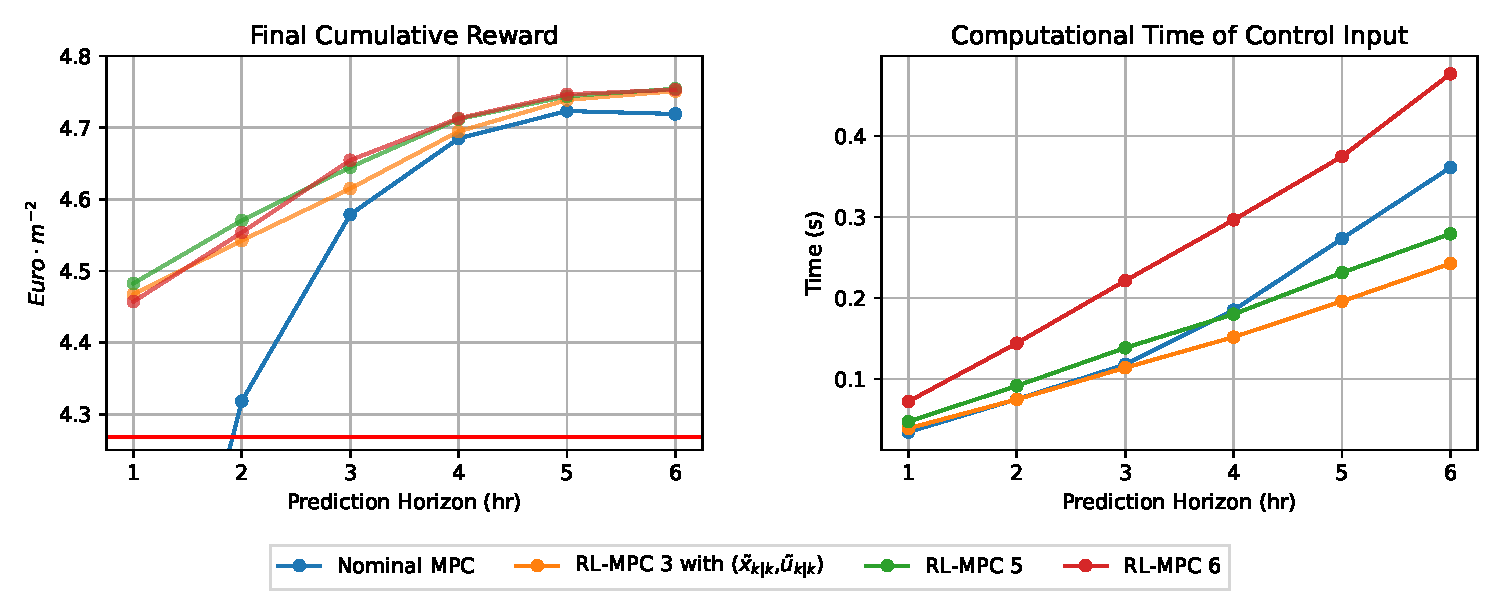
\includegraphics[width=\textwidth]{figures/rl_mpc_impl_final.pdf}
	\caption{MPC final }
	\label{fig:rlmpc-final}
\end{figure}

The final results of the mentioned implementations are shown in \autoref{fig:rlmpc-final}. While including a terminal region is the primary factor in improving performance, incorporating the value function can additionally enhance performance, albeit with the drawback of increased computational time. This suggests that the value function and terminal region provided by RL satisfy assumption 4 to ensure the performance of an EMPC. However, formal proof would be needed to confirm this conclusively. Moreover, the increase in computational time is not that extreme when a neural network is implemented, especially when adding a terminal region to aid the MPC in finding solutions faster. While the computational time increase may appear insignificant, this system is relatively uncomplicated compared to others. If this approach is used in highly complex systems, this increase in computational time could lead to large enough delays in the control input to destabilise the system. Therefore, any method to reduce the computational time is highly beneficial. Moreover, it seems that there is very little benefit to adding a cost function when the advantages of adding a terminal constraint are already so beneficial.


\begin{table}[H]
	\centering
	\renewcommand{\arraystretch}{1.3}
	\setlength{\tabcolsep}{8pt}
	\caption{Performance Comparison: RL-MPC 3 and 5 vs. MPC and RL}
	\label{tab:rlmpc-3-5-vs-MPC-and-RL}
	\resizebox{\columnwidth}{!}{%
		\begin{tabular}{ccccccccccc}
			\toprule
			& \multicolumn{2}{c}{1 hr} & \multicolumn{2}{c}{2 hr} & \multicolumn{2}{c}{3 hr} & \multicolumn{2}{c}{4 hr} & \multicolumn{2}{c}{5 hr} \\
			\cmidrule(lr){2-11}
			& Perf & Time & Perf & Time & Perf & Time & Perf & Time & Perf & Time \\
			\midrule
			RL-MPC 3 (\%) & 19.91 & 10.91 & 5.191 & 2.38 & 0.79 & -5.38 & 0.21 & -8.47 & 0.328 & -16.2 \\
			RL-MPC 5 (\%) & 20.32 & 24.26 & 5.84 & 18.26 & 1.44 & 44.37 & 0.57 & 3.68 & 0.435 & 2.71 \\
			\bottomrule
		\end{tabular}%
	}
\end{table}

\autoref{tab:rlmpc-3-5-vs-MPC-and-RL} displays the performance increase of RL-MPC 3 and RL-MPC 5 against the nominal MPC and a comparison with RL at a 1-hour prediction horizon. Incorporating a terminal region and value function offers minimal advantages compared to only using a terminal region, as the marginal improvement in performance results in a significantly larger increase in computational time. This reiterates the importance of reducing the computational cost of the neural network in the optimisation problem. As seen in \autoref{fig:rlmpc-final}, RL-MPC 6 offers promising results as an alternative method to using the value function and could yield even more benefits when more than two initial trajectories and terminal regions are provided by various agents and methods. The computational time of RL-MPC 6 can theoretically be halved by solving the problems in parallel, resulting in a compute cost similar to RL-MPC 3 and a similar performance to RL-MPC 5. Further research should be conducted on this implementation in the future.\\

While the combination of RL and MPC shows promising results, it is important to note that the simulations remain deterministic. These results primarily indicate which implementations are worth testing further in a stochastic environment to create a more accurate depiction of reality. Moreover, it may be tempting to use RL-MPC 2 (with terminal constraint) to guarantee performance as good as RL. However, this may not be practically achievable in a stochastic environment. Due to the randomness in the state evolution of a stochastic environment, it is impractical to ensure that the system can always meet the terminal point constraint exactly as defined by the reference trajectory. Consequently, allowing a terminal region constrain relaxes this constraint and makes the problem feasible. Finally, a value function derived from a policy that inherently considers uncertainty can provide the MPC with valuable insights regarding the impact of uncertainty on its calculated control actions. Therefore, RL-MPC 3 and RL-MPC 5 are suitable choices for testing in a stochastic environment. RL-MPC 6 was not tested on a stochastic environment for computational reasons; however, further research should be conducted to investigate its efficacy.

